\section{Dropping Policies}
\label{sec:policies}

In order to use partial monitoring to enable adjustable overheads, we must also
specify a policy for when and which monitoring events are dropped. In this
section, we discuss some of the options and trade-offs for dropping policies.
We split this decision into two components:
\begin{enumerate}
  \item When do we need to drop events in order to enable reduced overheads? (Section~\ref{sec:policies.when})
  \item Which events should be dropped? (Section~\ref{sec:policies.which})
\end{enumerate}

% Our goal with enabling partial monitoring is to allow for a specified overhead target or budget to be met while maximizing the amount of monitoring performed.
% This is done by dynamically dropping a portion of the monitoring operations. In this section, we discuss in detail how this dropping decision is
% made. Specifically, we first discuss how to decide when dropping should be performed 
% Section~\ref{sec:policies.slack}. Next, we investigate trade-offs created by
% selecting which events are dropped (Section~\ref{sec:policies.events}). Different policies in determining which
% events can be dropped create a trade-off between how closely the overhead
% budget is met and the monitoring coverage achieved.

\subsection{Deciding When to Drop}
\label{sec:policies.when}

% Slack
\begin{figure}
  \begin{center}
    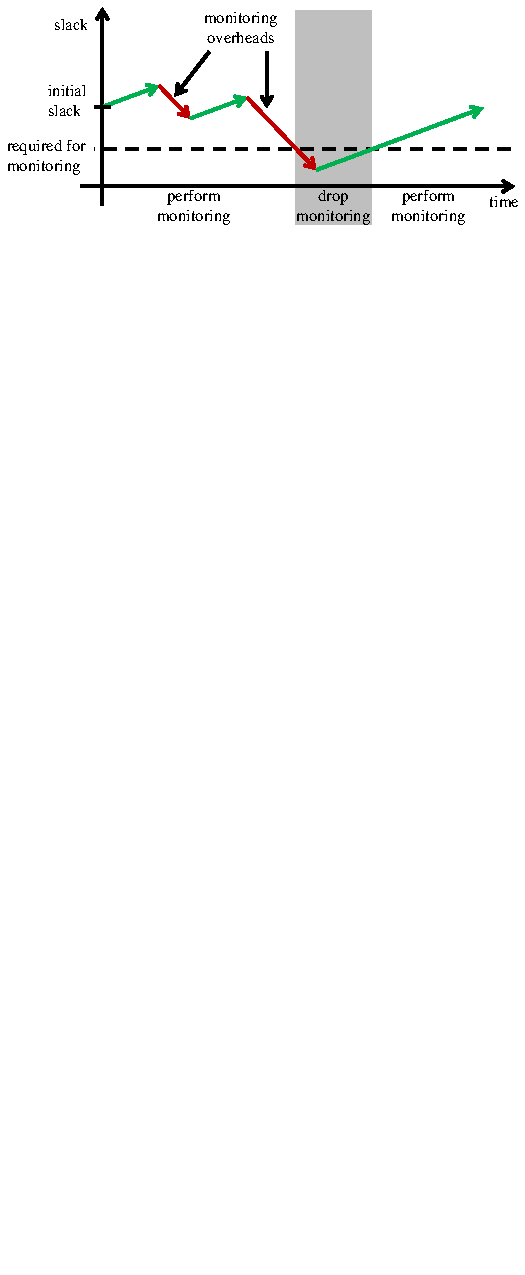
\includegraphics[width=\columnwidth]{figs/slack.pdf}
    \vspace{-0.2in}
    \caption{Slack and its effect on monitoring over time.}
    \label{fig:policies.slack}
    \vspace{-0.1in}
  \end{center}
\end{figure}

In this section, we discuss two possible ways to determine when events should be dropped.
The first possibility is to probabilistically drop events. By setting the probability of
dropping events appropriately, overheads can be reduced. This works well for
enabling partial monitoring for cooperative testing and debugging since the
randomness allows different users and runs to monitor different portions of the
program. However, using a probabilistic dropping policy can make it difficult
to meet a target overhead without prior profiling.

Alternatively, we can specify a target overhead and estimate, at run-time, the
overheads of monitoring in order to decide whether dropping is needed.
The overhead budget is specified as a percentage of the main program's execution
cycles without monitoring. In order to estimate overheads at run-time, we define \emph{slack} as the number of cycles of
monitoring overhead that can be incurred while staying within the budget
target. Slack is essentially the difference between the actual overhead seen
and the budget specified. Slack is generated as the main program runs and consumed as monitoring overheads occur.  For
example, if no monitoring overheads occur during 1000 cycles of the main
program's execution and the designer sets a 20\% overhead target, then the
slack that is built up during this period is 200 cycles. If the main core is
then stalled for 50 cycles due to monitoring, then the remaining slack is 150
cycles. 
In addition to this accumulated slack, a small amount of initial slack
can be given in order for monitoring to be performed at the start of a program.
Figure~\ref{fig:policies.slack} shows an example of how slack can change over time.
In this slack-based policy, if the slack falls below zero (i.e., the overhead budget is exceeded), then
monitoring events should be dropped.

% % Slack tracking module
% \begin{figure}
%   \begin{center}
%     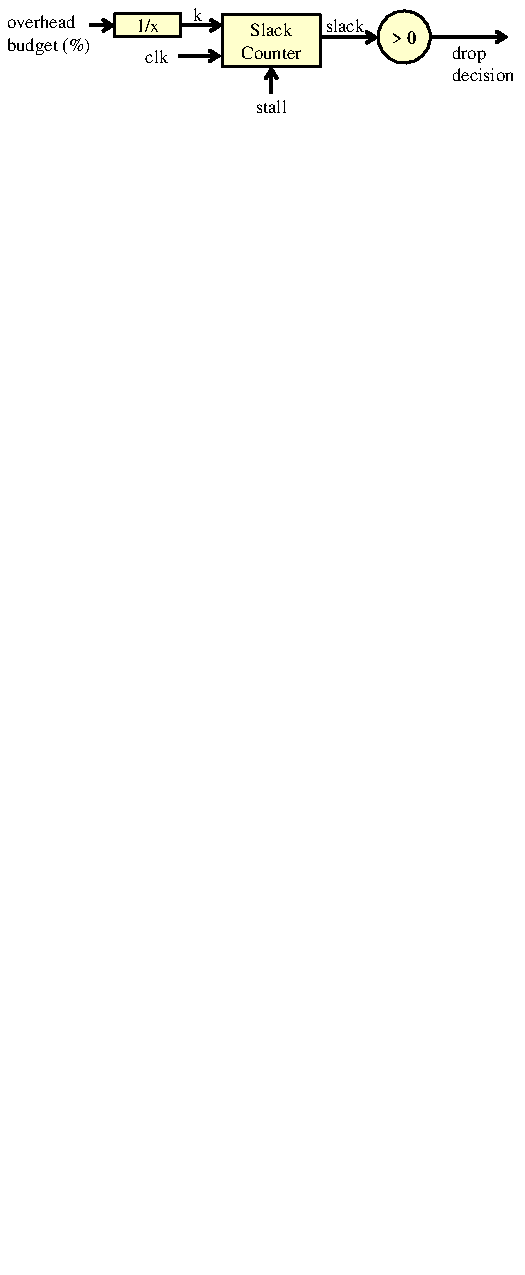
\includegraphics[width=\columnwidth]{figs/stm.pdf}
%     \vspace{-0.2in}
%     \caption{Slack tracking and drop decision hardware.}
%     \label{fig:policies.stm}
%     \vspace{-0.1in}
%   \end{center}
% \end{figure}

% Figure~\ref{fig:policies.stm} shows a hardware slack tracking module for
% keeping track of slack. 
Slack can be easily measured in hardware by using a counter that increments on every $k$-th
cycle of the main core (e.g., every 5th cycle for a 20\% target budget). 
% This $k$ can be calculated by taking the reciprocal of
% the target budget. For example, if the target budget is 20\%, then the counter
% increments on every 5th clock cycle. 
The value of this counter is the
accumulated slack. Whenever the main core is stalled due to the monitor, the
measured slack is decremented. It is difficult to precisely determine the
entire impact of monitoring on the main core due to the
difficulty in measuring certain overheads such as contention for shared memory.
However, we have found that using only the stalls due to FIFO back pressure
works well in practice.

\subsection{Deciding Which Events to Drop} 
\label{sec:policies.which}

% % Varying slack's impact on coverage for UMC
% \begin{figure}
%   \begin{center}
%     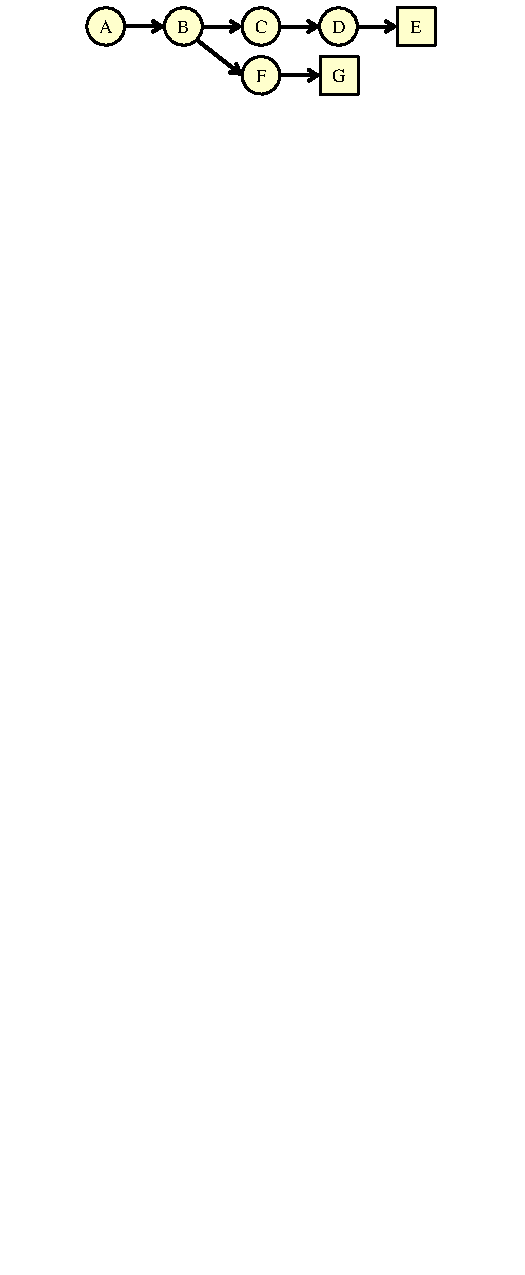
\includegraphics[width=\columnwidth]{figs/dataflow_graph.pdf}
%     \vspace{-0.3in}
%     \caption{Example dependence graph for metadata. Square nodes represent
%     events where checks are performed.} 
%     \label{fig:policies.dataflow_graph}
%     \vspace{-0.1in}
%   \end{center}
% \end{figure}

\begin{figure}
  \begin{center}
  \subfloat[Unrestricted Dropping]{
    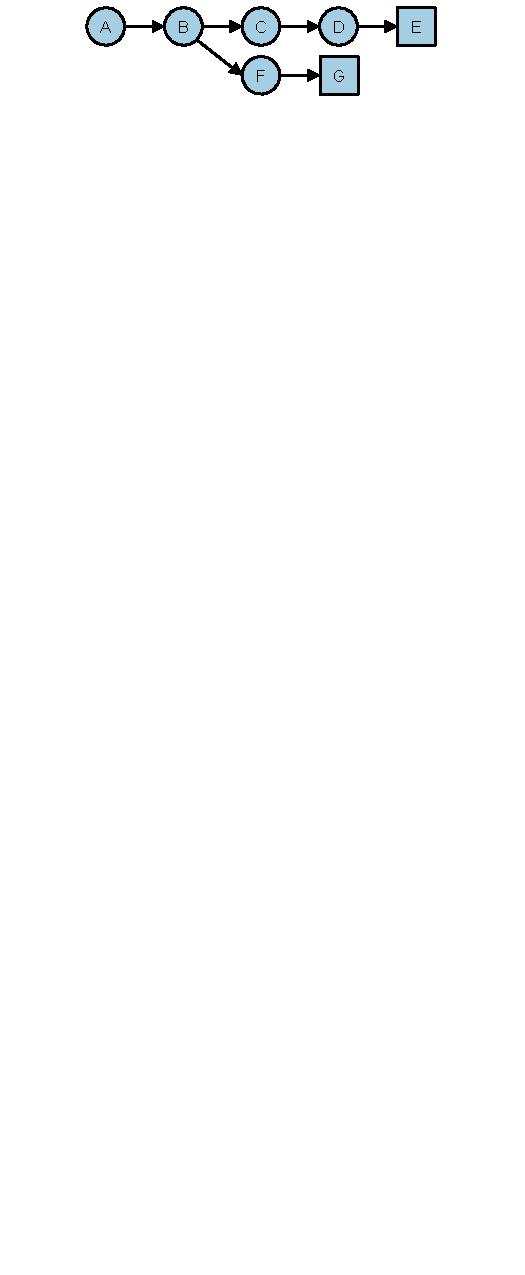
\includegraphics[width=\columnwidth]{figs/unrestricted_drop.pdf}
    \label{fig:policies.all_drop}
  }
  \vspace{-0.1in}
  \\
  \subfloat[Source-only Dropping]{
    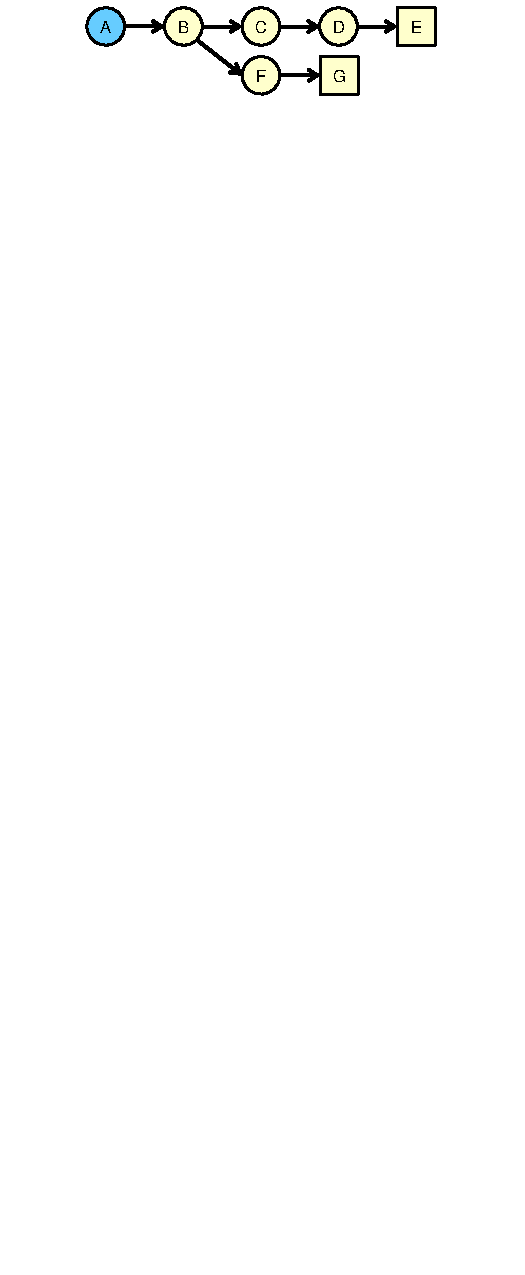
\includegraphics[width=\columnwidth]{figs/source_drop.pdf}
    \label{fig:policies.source_drop}
  }
  \vspace{-0.1in}
%   \\
%   \subfloat[sub-flow dropping]{
%     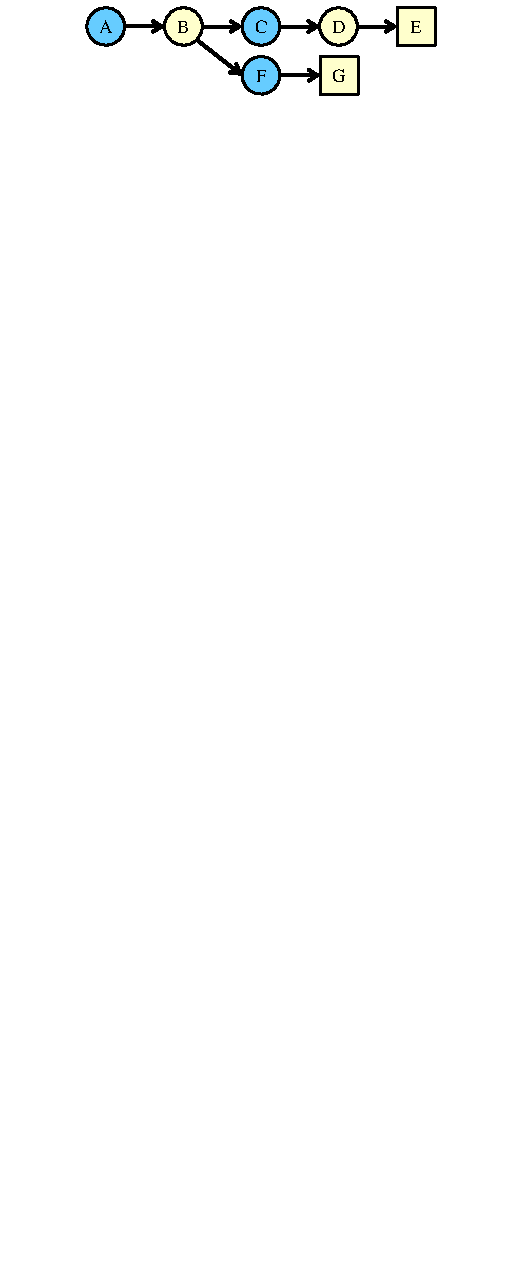
\includegraphics[width=\columnwidth]{figs/min_drop.pdf}
%     \label{fig:policies.min_drop}
%   }
  \end{center}
  \caption{Comparison of dropping policies using metadata dependence graphs.
  Square nodes represent events where check are performed. Blue (dark) nodes
  indicate which nodes can be dropped.}
  \label{fig:policies.policies}
\end{figure}

In addition to deciding when dropping is required, trade-offs also exist in
deciding which events should be dropped.
The simplest policy is to drop any monitoring events when slack is less than or equal to zero.  However, this can result in
wasted work. For example, consider the metadata dependence graph shown in
Figure~\ref{fig:policies.all_drop}. Here, an edge from node {\tt A} to node
{\tt B} represents that if event {\tt A} is dropped, then due to its
invalidated metadata, it will cause event {\tt B} to be dropped. Square
nodes indicate events where monitoring checks are performed. In the
example, suppose that event {\tt E} is meant to perform a check operation but is dropped.
In this situation, the
monitoring operations that were done for events {\tt C} and {\tt D} were wasted
since their results were not used for any monitoring checks.
That is, by the time we decide to drop event {\tt E}, we have already 
updated metadata due to events {\tt C} and {\tt D} even though they are no longer needed.

An alternative dropping policy which eliminates this wasted work is to only make dropping decisions at
the root or source of these metadata flows. That is, we will decide to either monitor or
not monitor an entire metadata flow. An example of these source nodes is the
monitoring done to initialize base and bounds information on {\tt malloc} for
an array bounds check. We refer to this dropping decision policy
as \emph{source-only dropping} and we refer to the previous policy of 
dropping any event as \emph{unrestricted dropping}.

Figures~\ref{fig:policies.all_drop} and \ref{fig:policies.source_drop} show a
comparison of where dropping decisions are made for these two policies. Source
dropping will
result in no wasted work and thus better coverage. However, because of the coarser-grained decision, it
may be more difficult to closely match overheads. We expect source-only dropping 
to work well when there are a large number of independent metadata flows.
In addition, using a probabilistic dropping policy works poorly with
unrestricted dropping. Since each event in a dependent chain (e.g., events {\tt
A} through {\tt E}) needs to be monitored in order for the monitoring check to
be useful, randomly dropping any event will cause the final check to be
invalid.

Depending on the target application of partial monitoring, different policies
are more applicable.
For applications where closely matching an overhead target is important, a
slack-based, unrestricted dropping policy is appropriate. However, if matching
the overhead target is not as important, then a slack-based, source-only dropping
policy could provide better coverage. 
Finally, if the goal is to use partial monitoring to enable cooperative
debugging and testing with very low overheads, then a probabilistic,
source-only dropping policy can be used to provide good total coverage over
multiple runs.

% Trade-off between source-drop and unrestricted dropping
% \begin{figure}
%   \begin{center}
%     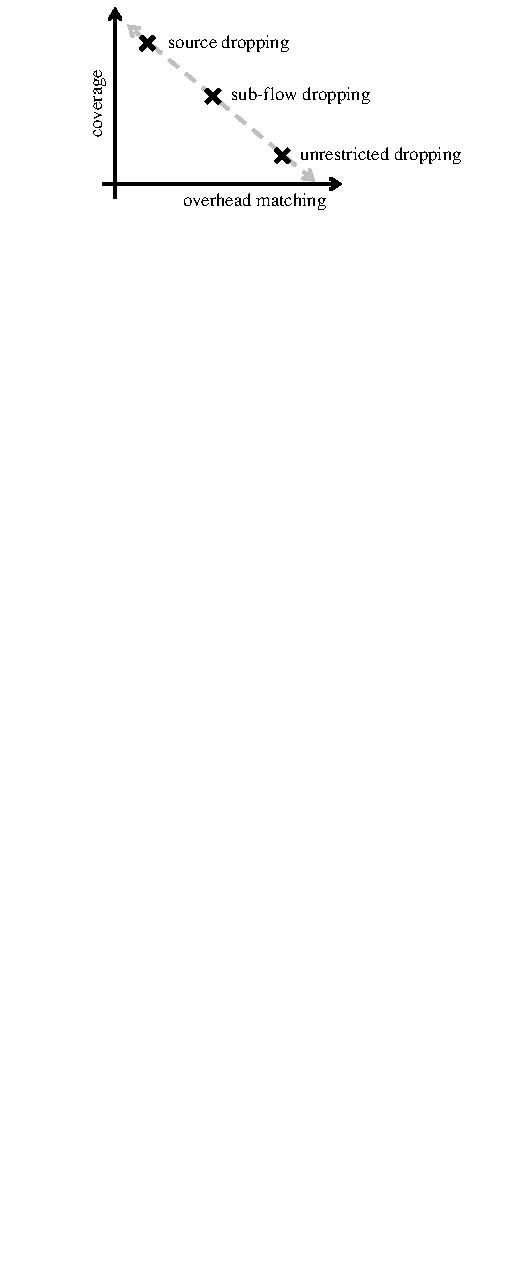
\includegraphics[width=\columnwidth]{figs/policy_trade_off.pdf}
%     \vspace{-0.3in}
%     \caption{Slack tracking and drop decision hardware.}
%     \label{fig:policies.trade_off}
%     \vspace{-0.2in}
%   \end{center}
% \end{figure}
% 
% Another possible method is to make the dropping decisions somewhere in between
% source-only dropping and unrestricted dropping. From the graph in 
% Figure~\ref{fig:policies.dataflow_graph}, we can see that if the dropping
% decision is made at event {\tt C} then we can skip event {\tt E} with no wasted
% work. If we instead choose to perform monitoring for event {\tt C}, then we want to perform all
% monitoring on that flow. Similarly, event {\tt F} creates a decision point for
% the bottom flow that will result in no wasted work and dropping event {\tt A}
% allows the entire shown metadata flow to be dropped with no wasted work. If the
% program can be
% analyzed or profiled to identify these instructions which, if dropped, lead to
% no wasted work, then this information can be used at run-time to minimize the
% amount of wasted work. We refer to this policy as \emph{sub-flow dropping}.
% Figure~\ref{fig:policies.min_drop} shows the points were dropping decisions are
% made for this policy.
% Sub-flow dropping is a coarser-grained decision than unrestricted dropping, but
% finer-grained that source-only dropping. Thus, its ability to match overheads is
% expected to sit between these other two policies. Similarly, there still exists
% edge cases where wasted work can occur, but typically we expect much less
% wasted work than unrestricted 
% dropping. Thus, we expect the coverage achieved by sub-flow dropping for a
% certain overhead to fall between source-only and unrestricted dropping. These three
% dropping policies create a trade-off space between coverage achieved and
% ability to match an overhead target.
% Figure~\ref{fig:policies.trade_off} summarizes this trade-off between coverage
% and ability to match overhead.
